\documentclass{article}
\usepackage[T1]{fontenc}
\usepackage[utf8]{inputenc}
\usepackage{amsmath, amssymb}
\usepackage{tikz}
\usepackage{tikzsymbols}
\usepackage{wasysym} %for the notes
\usepackage{lmodern}
\usepackage{xcolor}
\usetikzlibrary{arrows,automata}
\setlength\parindent{0pt}

\begin{document}

\begin{center}
  \Large{Informatik D - Übungsblatt 4}

  \large{Sebastian Höffner, Andrea Suckro}
\end{center}



\section*{Aufgabe 4.1}
Automat zur Addition zweier Binärzahlen.
\begin{center}
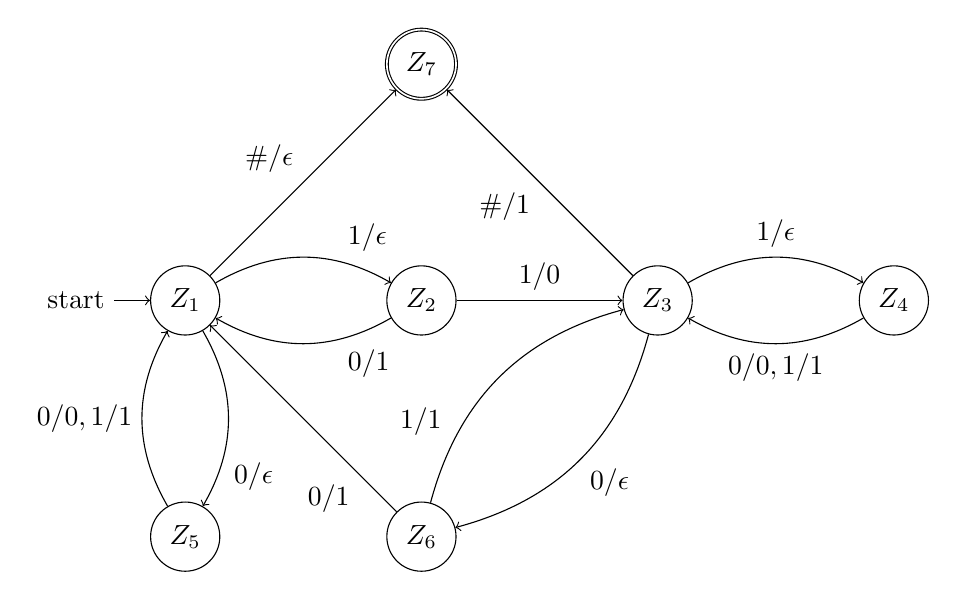
\begin{tikzpicture}[->, auto, node distance=3cm]
  \node[initial,state]   (Z1)               {$Z_1$};
  \node[state]           (Z2) [right of=Z1] {$Z_2$};
  \node[state]           (Z3) [right of=Z2] {$Z_3$};
  \node[state]           (Z4) [right of=Z3] {$Z_4$};
  \node[state]           (Z5) [below of=Z1] {$Z_5$};
  \node[state]           (Z6) [below of=Z2] {$Z_6$};
  \node[state,accepting] (Z7) [above of=Z2] {$Z_7$};

  \path (Z1) edge [bend left, pos=0.7] node {$0/\epsilon$} (Z5)
  	  	  	 edge [bend left, pos=0.7] node {$1/\epsilon$} (Z2)
             edge                      node {$\#/\epsilon$}(Z7)
        (Z2) edge [bend left, pos=0.3] node {$0/1$}        (Z1)
             edge                      node {$1/0$}        (Z3)
        (Z3) edge [bend left]          node {$0/\epsilon$} (Z6)
             edge [bend left]          node {$1/\epsilon$} (Z4)
             edge                      node {$\#/1$}       (Z7)
  	  	(Z4) edge [bend left]          node {$0/0, 1/1$}   (Z3)
  	  	(Z5) edge [bend left]          node {$0/0, 1/1$}   (Z1)
        (Z6) edge [pos=0.2]            node {$0/1$}        (Z1)
             edge [bend left, pos=0.2] node {$1/1$}        (Z3)
        ;
\end{tikzpicture}
\end{center}


\section*{Aufgabe 4.2}

\section*{Aufgabe 4.3}
\subsection*{a)}
Wir nehmen an $L_1=\left\{\eighthnote^i\halfnote^{2i} | i \geq 0\right\}$ sei regulär, damit gelte für $L_1$ das Pumping Lemma. Sei $n$ die entsprechende Wortmindestgröße. Dann betrachten wir das Wort $z=\eighthnote^n\halfnote^{2n} \in L_1$. Es existiert nun eine Zerlegung $uvw=z$ für die gilt:

\begin{align}
|v| = l &\geq 1\\
|uv| &\leq n\\
\eighthnote^{n-l}\halfnote^{2n} &\notin L_1
\end{align}

$\eighthnote^{n-l}\halfnote^{2n}$ kann nicht in $L_1$ liegen, da $2(n-l) = 2n$ nur gilt wenn $l=0$ ist, was allerdings nach (1) nicht erfüllt ist. $L_1$ ist somit nicht regulär.
\setcounter{equation}{0}

\subsection*{b)}
Wir nehmen an $L_2=\left\{\eighthnote^i\halfnote^j | 0\leq i \leq j\right\}$ sei regulär, damit gelte für $L_2$ das Pumping Lemma. Sei $n$ die entsprechende Wortmindestgröße. Dann betrachten wir das Wort $z=\eighthnote^n\halfnote^j, j = n + x, x \geq 0 \in L_2$. Wobei $x$ den Unterschied in der Länge zwischen $i$ und $j$ repräsentiert. Es existiert nun eine Zerlegung $uvw=z$ für die gilt:

\begin{align}
|v| &\geq 1\\
|uv| &\leq n\\
\eighthnote^{n+x+1}\halfnote^{j} &\notin L_2
\end{align}

$\eighthnote^{n+x+1}\halfnote^{j}$ sollte nach dem Pumping Lemma in $L_2$ liegen, kann es allerdings nicht, da $n+x+1 > j $ ist. $L_2$ ist somit nicht regulär.
\setcounter{equation}{0}

\subsection*{c)}
Wir nehmen an $L_3=\left\{\quarternote^{k^2}| k\geq0 \right\}$ sei regulär, damit gelte für $L_3$ das Pumping Lemma. Sei $n$ die entsprechende Wortmindestgröße. Dann betrachten wir das Wort $z=\quarternote^{n^2} \in L_3$. Es existiert nun eine Zerlegung $uvw=z$ für die gilt:



\section*{Aufgabe 4.4}

\section*{Aufgabe 4.5}

\section*{Aufgabe 4.6}
Wenn die Sprache regulär ist, dann können wir z.B. einen endlichen Automaten oder regulären Ausdruck finden, der diese Sprache beschreibt.

\subsection*{Regulärer Ausdruck}
In Übung 2 haben wir $\Smiley^x$ verwendet, um $x$ wiederholungen von $\Smiley$ darzustellen. Mit der gleichen Schreibweise können wir die Sprache $\mathbb{L}$ als regulären Ausdruck darstellen:

\begin{align*}
a^0a^*b^0|a^1a^*b^1|a^2a^*b^2|...|a^{2000}a^*b^{2000}
\end{align*}


\end{document}